\documentclass{math}

\usepackage{float}
\usepackage{geometry}
\usepackage{graphicx}
\usepackage{listings}
\usepackage{subcaption}

\geometry{letterpaper, margin=0.25in}

\title{Principles of Data Management}
\author{Insert Group Name Here}
\date{August 2018 - December 2018}

\begin{document}

\lstset{basicstyle=\ttfamily\footnotesize,breaklines=true}
\maketitle

\section*{Phase 2}
Our application software will be in the form of a command line interface that
provides a tree of commands to the user. The intended user of this software will
be administrators who can access information related to customers, dealers,
vehicles, and the relationships between them. This software can also function
as an abstraction of the database to developers who need access to a higher
level API that can provide information about the relationships between
customers, dealers, and vehicles.

\subsection*{ER and UML Diagrams}
\begin{figure}[H]
  \centering
  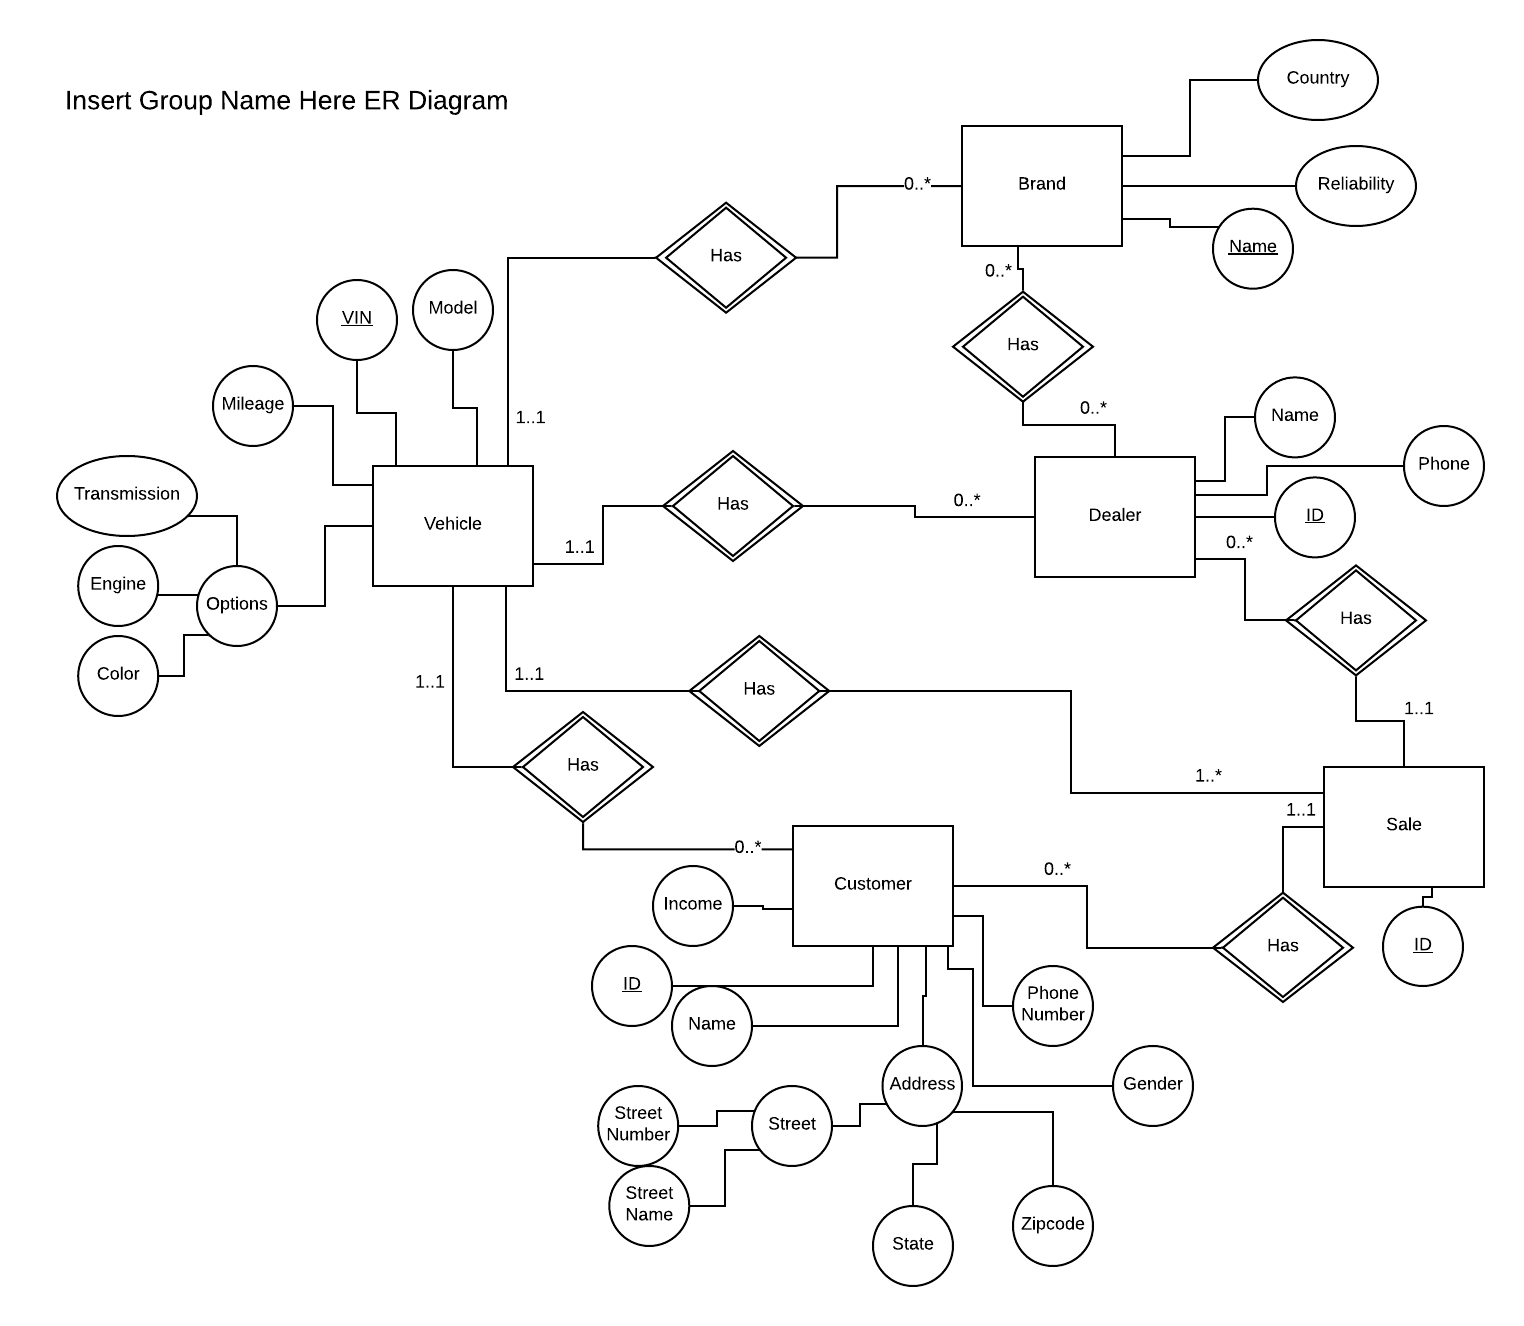
\includegraphics[width=20cm]{assets/phase2_er_diagram.png}
  \caption{ER diagram}
\end{figure}
\begin{figure}[H]
  \centering
  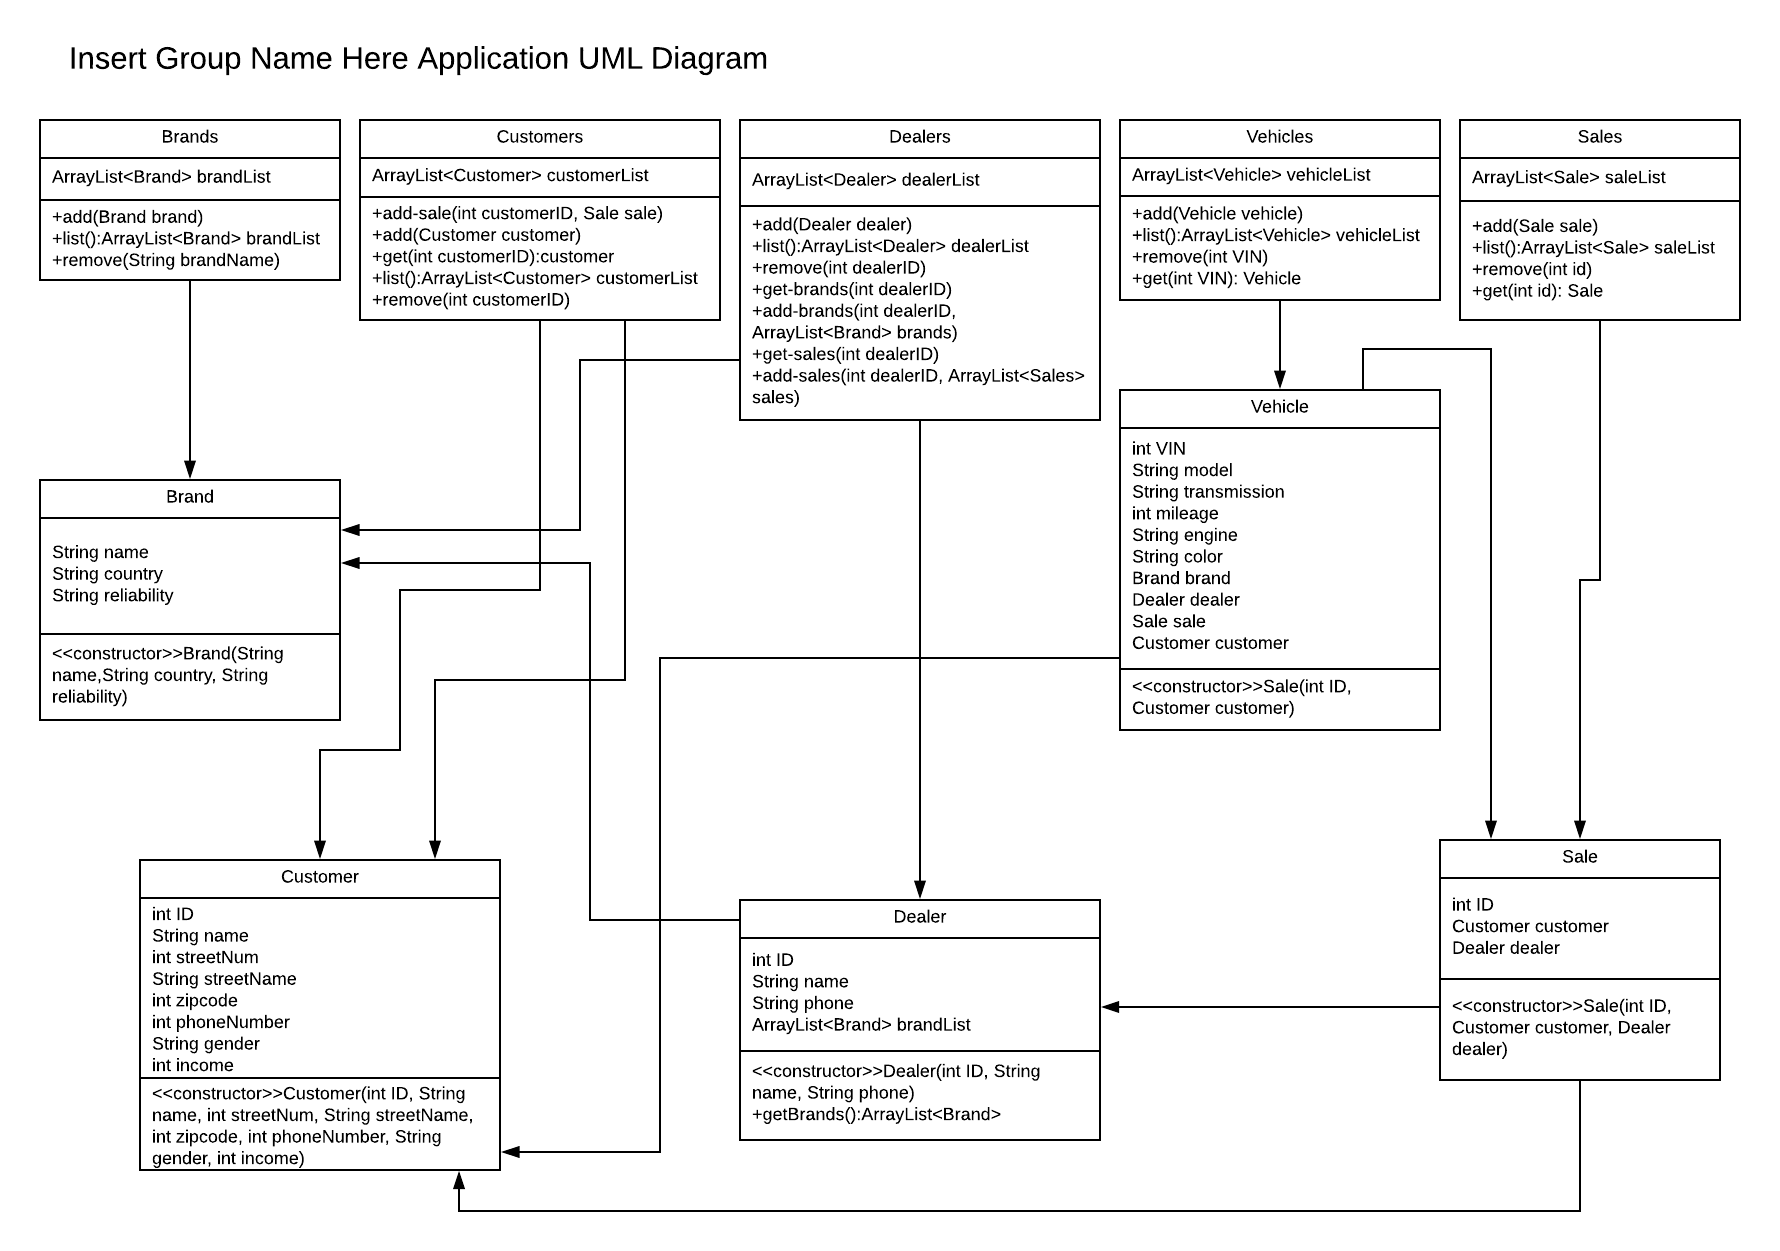
\includegraphics[width=20cm]{assets/phase2_uml_diagram.png}
\end{figure}

\subsection*{Application Software}
The user interface will be a command line interface using a tree of commands
that allow access to customers, dealers, vehicles, and information related to
the relationships between them.
\begin{figure}[H]
  \centering
  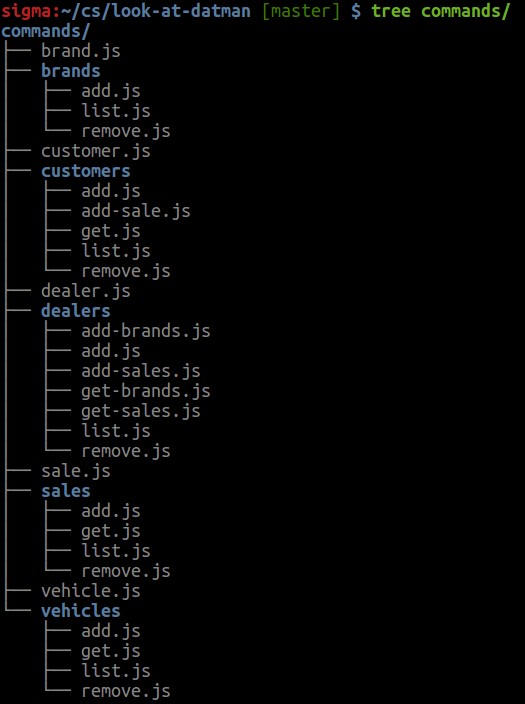
\includegraphics[width=8cm]{assets/phase2_command_tree.png}
  \caption{Minimal command tree of available actions}
\end{figure}
\begin{figure}[H]
  \centering
  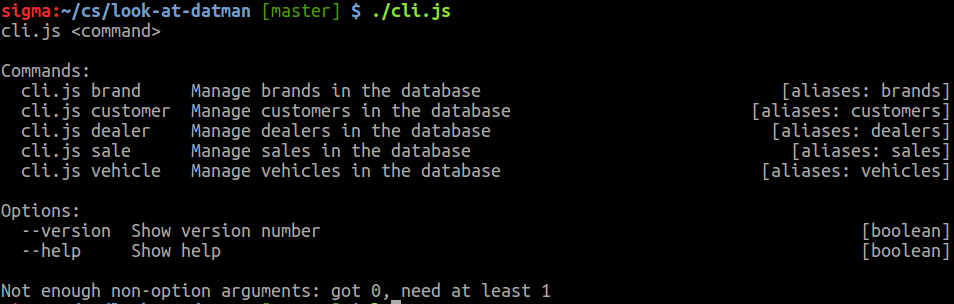
\includegraphics[width=18cm]{assets/phase2_manpage.png}
  \caption{CLI help prompt}
\end{figure}
The CLI will internally handle formatting and assembling more complicated
queries before executing it on the database. It will directly query the database
with relevant queries to fetch data for display. The user-facing input side of
the software (argument capturing, command line flags, command tree) is handled
by the \texttt{yargs.js} package while the table display formatting is handled
by the \texttt{cli-table3} package (both available on npmjs).

\subsection*{Use Cases}
This application's intended users are data administrators and developers who
will use this as an API. Database functionality will be abstracted away into
our application so that users can provide simple queries and commands to
perform common actions such as executing a sale, searching up dealers, or
registering users. This application will likely be used as a backbone in
external point-of-sale software or invoked directly from the command line by
an administrator.

\subsection*{Sample SQL}
Creating the tables:
\begin{lstlisting}
create table if not exists customer (
  id int primary key,
  income int,
  name varchar(255),
  phone varchar(255),
  gender varchar(16),
  address_street varchar(255),
  address_state varchar(255),
  address_zipcode varchar(255)
);

create table if not exists dealer (
  id int primary key,
  name varchar(255),
  phone varchar(255)
);

create table if not exists brand (
  name varchar(255) primary key,
  country varchar(255),
  reliability varchar(255)
);

create table if not exists sale (
  id int primary key,
  customer int references customer(id),
  dealer int references dealer(id)
);

create table if not exists vehicle (
  vin int primary key,
  model varchar(255),
  transmission varchar(255),
  mileage int,
  engine varchar(255),
  color varchar(255),
  brand varchar(255) references brand(name),
  dealer int references dealer(id),
  sale int references sale(id),
  customer int references customer(id)
);

create table if not exists brand_dealer (
  brand varchar(255) references brand(name),
  dealer int references dealer(id)
);
\end{lstlisting}
Fetching all vehicles purchased by a customers in NY:
\begin{lstlisting}
select model,brand from vehicle where customer in
  (select id from customer where address_state = "NY");
\end{lstlisting}
Set a brand's reliability:
\begin{lstlisting}
update brand set reliability="poor" where name="Ford";
\end{lstlisting}
Add a new vehicle for a dealer:
\begin{lstlisting}
insert into vehicle values(
  1243, "Accord", "Automatic", 10000, "V6", "Ugly", "Honda", 3, NULL, NULL)
\end{lstlisting}

\subsection*{User Interface}
If a query is executed via the command line, the data returned will be nicely
formatted into a terminal compatible table for display.
\begin{figure}[H]
  \centering
  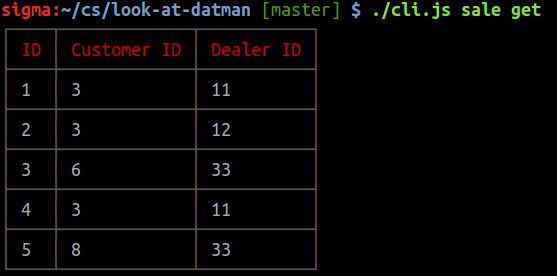
\includegraphics[width=10cm]{assets/phase2_example_table.png}
  \caption{Formatted table in terminal}
\end{figure}
Configuration data and query parameters will be specified by command line
arguments or flags for relevant commands.

\subsection*{Sample Data}
Included in the project zip as CSVs.

\subsection*{Attributes Domain}
Vehicle:
\begin{itemize}
  \item Vin: A unique identification code consisting of a combination of 17
    numbers and capital letters. The domain is any combination of numbers and
    letters totaling 17 characters. Is the primary key for Vehicles.
  \item Options: Consists of three other attributes: Engine, Color and
    Transmission. This consists of any three combinations of the previous
    attributes.
  \item Engine: Type of engine that the car has, this domain is any kind of
    engine that is used in cars i.e. (VEE, INLINE, STRAIGHT, etc).
  \item Color: This is the color of the car, as stated it is any word that
    accurately describes the color of the car (black, grey, blue, etc).
  \item Transmission: Type of transmission the car has, this domain is any type
    of transmission a car may have (Automatic, Manual, Dual-Clutch, etc).
  \item Model: The exact model of the car, can be any valid car model which is
    a collection of characters, ie (Camry, Highlander, Enclave, etc).
  \item Mileage: The mileage that the car has traveled, will be an integer that
    is usually 4 to 7 digits.
\end{itemize}
Dealer:
\begin{itemize}
  \item ID: Unique identifier for the dealer will be a unique combination of
    letters and numbers. Is the primary key for Dealers.
  \item Name: Name of the dealer can be any combination of characters.
  \item Phone: Phone number for the dealer can be any valid phone number,
    meaning a three-digit area code and a seven-digit number.
\end{itemize}
Brand:
\begin{itemize}
  \item Country: Country of origin for the brand, will be the name of any
    country which can be any combination of characters.
  \item Reliability: Adjectives describing the reliability of the brand, domain
    will be (Great, Fair, Poor).
  \item Name: The name of the brand itself. It can be any combination of
    letters and will be used as the primary key for Brand.
\end{itemize}
Sale:
\begin{itemize}
  \item ID: Unique identifier for the sale will be a unique combination of
    letters and numbers and will be used as the primary key of Sales.
\end{itemize}
Customer:
\begin{itemize}
  \item ID: Unique identifier for the customer, will be a unique combination of
    letters and numbers and is the primary key of Customer.
  \item Name: Will be the full name of the customer, which can be any
    combination of letters.
  \item Address: Address of the customer, will be any valid address string
    consisting of the street address, state and zip code.
  \item Street: The street address of the customer this includes the street
    name and the number.
  \begin{itemize}
    \item Street Number: The street number will be the street number of the
      customer, this will be a combination of numbers.
    \item Street Name: The name of the street the customer lives on, will be a
      combination of letters containing its suffix.
    \item Zip code: Represents the zip code the customer lives in, will be
      six-digits long.
  \end{itemize}
  \item Phone Number: This is the customers given phone number, domain will be
    any valid phone number, meaning that it’s a 10 digit number consisting of
    the 3 digit area code and their number.
  \item Gender: Will be the gender of the customer, it will be a single letter
    representing the gender.
  \item Income: The customer’s annual income, typically a number between 5-8
    digits.
\end{itemize}

\begin{center}
  You can find all my notes at \url{http://omgimanerd.tech/notes}. If you have
  any questions, comments, or concerns, please contact me at
  alvin@omgimanerd.tech
\end{center}

\end{document}
